Stochastic systems have been used extensively in several areas including  verification~\cite{FKNP11}, learning theory~\cite{AJKS21}, epidemic processes~\cite{Lef81} to name a few. Several real-world systems however do not work with a centralised control. Therefore, modelling using stochastic systems with multiple agents makes for more faithful abstractions of such systems without a centralised control. Some examples of fields in which multi-agents stochastic modelling include cyber physical systems~\cite{SEC16}, distributed and probabilistic computer programs~\cite{dAHJ01}, probabilistic planning~\cite{TKI10}. In such cases, the problem of reasoning about multiple agents with several, often times orthogonal objectives, becomes important. % However, for situations that are modelled as graph games, Nash equilibria come with its own down-sides and therefore several notions of equilibria have emerged in turn-based games on graphs to circumvent the problems posed by the natural definitions of Nash equilibira, like subgame-perfect equilibira, Stackleberg-equilibria. 
For multi-agent systems modelled with stochasticity on the underlying arena, a fundamental question to ask is the existence or finding of an equilibrium.
The most popular equilibria in literature are Nash equilibria~\cite{Nas50}. However, those come with their own downsides. The computational complexity for studying Nash equilibria over multi-agent systems is prohibitively expensive, and even undecidable in the general case, where systems have $10$ or more players~\cite{UW11}. 
Further, even if Nash equilibria could be computed efficiently, they do not faithfully model the agents in real world settings
%as each agent might perceive risk differently. With randomness arising from both the strategies of other agents, as well as the underlying model of the system, this might mean that risk-averse or risk-loving agents might have an incentive to deviate since their perceived values of outcome is different from expected value of the game.
since they do not consider their tolerance or averseness to risk.

Let us consider a $1$-player game where a protagonist is proposed two options: (a) earning \$1; (b) playing a lottery in which, with probability $\frac{1}{40}$, she gets \$40, and with probability $\frac{39}{40}$, she does not earn anything.
Classically, rational strategies would be maximising the expected payoff. From this perspective, both options yield an expected payoff of \$1, making them equivalent.
This approach is particularly justified when the game represents a scenario that can be repeated many times: the law of large numbers ensures that, in the long run, the average payoff will converge to the expected payoff. However, when the game is played only once, the protagonist may prioritise immediate needs. If she urgently requires \$1, the guaranteed option (a) becomes preferable.

Conversely, if she is a risk-taker or finds herself in a situation where only the \$40 can make a significant difference, she may prefer the high-risk option (b).
Although this choice might appear irrational, it mirrors the behaviour of millions of people who participate everyday in games with a negative expected payoff, driven by the allure of a potentially life-changing win, and generating an annual turnover of USD 536 billions~\cite{GamblingNewspaper23} for the gambling industry.
That industry, on the other hand, operates on a large scale where expected payoff becomes the key metric. 
This contrast underscores the importance of alternative measures to expected payoff that account for each agent's risk tolerance.%, offering a more nuanced understanding of decision-making in uncertain scenarios.

%We thus have an example of a two-player interaction, with apparently zero-sum payoffs, but where both players express a preference for the same option, because the context gives them a different tolerance to risk: this paradox underscores the importance of alternative measures to expected payoff that account for an agent's risk tolerance, offering a more nuanced understanding of decision-making in uncertain scenarios.
% This contrast underscores the relevance of generalising the notion of Nash equilibria: in a multi-agent system, the agents may have diverging perception of which risks can be taken.
% It makes sense, then, to study \emph{risk-sensitive equilibria}, in which players do not necessarily maximise their expected payoff, but their perception of what their payoff will be according to different risk measures.\leon{I'm actually not satisfied with this, I will modify it and move it.}


% Classically, we consider that a rational strategy would consist in maximising the expected payoff: from that perspective, the two choices are equivalent.
% Such an approach is justified especially when the game models a situation that can be repeated a large number of times, in which case the law of large numbers guarantees that the average payoff converges to the expected payoff.
% But when the game models a situation that is played only once, the protagonist may consider that she really needs her euro, and that the possibility of earning 40\$ is too unlikely to be taken into account: she would then have a justifiable preference for the option (a).
% On the contrary, if she is more of a gambler, or if she finds herself in a desperate situation in which only earning those 40\$ could save her, she could go all out and express a strict preference for option (b)\footnote{Even though this case seems more irrational, it explain why millions of people play everyday games in which they know that their expected payoff is negative.
% On the other side, the companies with whom they interact repeat the experience often enough to consider expected payoff as the relevant measure --- generating a yearly turnover of 536 billions of US\$.}.
% Hence the relevance of alternatives to expected payoff, that take into account the tolerance of the agent to risk.

\subparagraph*{Risk Measures.}
A \emph{risk measure} captures the perception that a player has of what their payoff will be. In that sense, they generalise the notion of expected payoff.
Various risk measures exist in the literature, and have been used extensively in the field of economics and finance. 
Some of these risk measures include expected shortfall (ES), value at risk (VaR)~\cite{Aue18}, variance~\cite{Bra99}, entropic risk measure (ER)~\cite{FS02}. 

%However, since the introduction of the characteristic of risk measure called \emph{coherence}~\cite{ADJH99}, it was expected that a ``good'' a risk measure must be coherent. A risk measure is coherent if it is monotonic, homogeneous, translational-invariance, and sub-additive.
%This automatically weeds out several of the above risk measures listed above like  Value at Risk or variance as a risk measure. 
A lot of work has been done in considering these risk measures over MDPs which use variance (along with mean) as a risk-measure~\cite{FK89, PSB22,MT11}, ES~\cite{RRS15,KM18,Meg22} (also referred to as conditional value at risk (CVaR), average value at risk (AVaR), expected tail loss (ETL), and superquantile in literature) and ER~\cite{HM72,BR14,BCMP24}. % have also been studied. 
Studying the entropic risk measure in MDPs appears more practical compared to expected shortfall  or using variance-penalised risk-measures. This impracticability of ES and variance-penalised measure in particular is due to the intractable exponential memory~\cite{HK15} and time required to compute optimal strategies~\cite{PSB22}, even for the one agent system of Markov decision processes (MDPs). On the other hand, when the risk measure used is ER, players have optimal positional strategies in MDPs~\cite{How72}, which makes it a prime candidate for consideration in multi-agent settings.

\subparagraph*{Entropic Risk Measure.}
The entropic risk measure is computed by assigning to each agent a risk parameter, i.e., a value $\rho \in \Rb$.
%Based on this risk parameter $\rho$, this measure first computes the expectation of the exponential function of the random variable and then re-normalises this.  
The entropic risk measure of a random variable $X$ is then defined as
$\re_\rho[X] = -\frac{1}{\rho} \log_e \left( \Eb \left[ e^{-\rho X}\right] \right)$. 
%For computational reasons, instead of the Euler's constant $e$, we use different bases sometimes.
If the risk parameter $\rho$ is positive, then more weight will be given to the bad payoffs: the corresponding player can then be considered as risk-averse.
Conversely, players with a negative $\rho$ are more risk-loving.
When $\rho$ tends to $0$, the entropic risk measure converges to the classical expectation $\Eb[X]$.

The game depicted by Figure~\ref{fig:example_gamma} extends the lottery example we discussed earlier. 
Black vertices are stochastic, and the circle vertex is controlled by player $\Circle$.
A play can be seen as an infinite sequence of moves of a token along the edges of the graph, starting from $a$: from a stochastic vertex, it takes one of the outgoing edges with the probabilities indicated on those, and from a vertex controlled by the player, she chooses which edge it takes.
The payoff $40$, $0$, or $1$ is obtained when the terminal vertex $t_1$, $t_2$, or $t_3$ is reached, respectively.
If no terminal vertex is reached, then the payoff is $0$.
Taking the red edge corresponds to option (a): then, her risk entropy is always $1$, for every risk parameter $\rho$.
But if she chooses option (b), that is, if she takes the blue edge, her risk entropy is $\re_\rho[\mu_{\circ}] = -\frac{1}{\rho} \log \left( \Eb \left[ e^{-\rho \mu_{\circ}}\right] \right) = -\frac{1}{\rho} \log \left(  e^{-40\rho } + \frac{39}{40} \right)$.
Both cases are illustrated with red and blue curves in \cref{fig:example_plot}.
The curves cross at abscissa $\rho = 0$, where the entropic risk measure corresponds to the expectation. Note that other strategies are possible if \emph{randomisation} is allowed---the player could, for example, toss a coin and participate in the lottery if the outcome is heads. The perceived reward of randomising between outermost red and blue edges are illustrated in the intermediate cases with mixtures of red and blue in \cref{fig:example_plot}.

%For this example, we  replace Euler's constant $e$ with instead the constant $2$, which makes $\re_\rho[X] = -\frac{1}{\rho} \log_2 \left( \Eb \left[ 2^{-\rho X}\right] \right)$.

%Player $\Circle$ gets the payoff $11$ if she reaches the terminal vertex $t_1$, the payoff $1$ if she reaches $t_2$, the payoff $2$ if she reaches $t_3$, and the payoff $0$ if she reaches none of those terminal states (i.e., if she loops on the vertex $a$ forever).

%If the player's strategy is to choose the red edge, she gets payoff $1$ with probability $1$.
%Therefore, her risk measure is equal to $1$ for every risk parameter $\rho$.

%If her strategy is to choose the blue edge going to $c$, then she gets the payoff $11$ with probability $\frac{1}{10}$, and $1$ with probability $\frac{9}{10}$.
%Thus her risk entropy is
%$\re_\rho[\mu_{\circ}] = \frac{1}{\rho} \log_2\left(\frac{1}{3} 2^{-4\rho} + \frac{2}{3} 2^{-1\rho}\right)$.
 
\begin{figure}[h] 
			\centering
            \begin{subfigure}[t]{0.4\textwidth}
			\begin{tikzpicture}[->,>=latex,shorten >=1pt, initial text={}, scale=1, every node/.style={scale=1}]
				\node[initial left, stoch] (a) at (0, 0) {$a$};
				\node[state] (b) at (1.5, 0) {$b$};
                \node[stoch] (c) at (2.5, 1) {$c$};
                \node (t1) at (4, 2) {$t_1:~\stack{\circ}{40}$};
                \node (t2) at (4, 0) {$t_2:~\stack{\circ}{0}$};
                \node (t3) at (3, -1) {$t_3:~\stack{\circ}{1}$};
                \path (a) edge[loop above] node[above] {$\frac{1}{2}$} (a);
				\path (a) edge node[above] {$\frac{1}{2}$} (b);
                \path (b) edge[blue, thick] (c);
                \path (b) edge[red, thick] (t3);
				\path (c) edge node[above] {$\frac{1}{40}$} (t1);
				\path (c) edge node[below] {$\frac{39}{40}$} (t2);
			\end{tikzpicture}
			\caption{A stochastic MDP}
			\label{fig:example_gamma}
            \end{subfigure}
            \begin{subfigure}[t]{0.55\textwidth}
			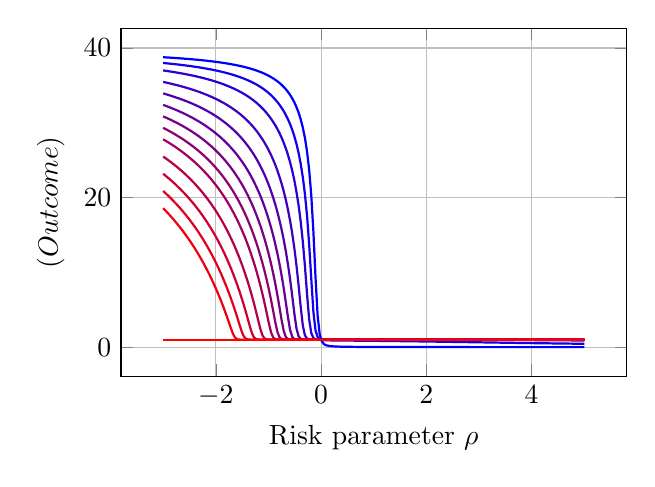
\begin{tikzpicture}
              \begin{axis}[
                xlabel={Risk parameter $\rho$},
                ylabel={$\re(\text{Outcome})$},
                domain=-3:5,
                samples=200,
                    width=8cm,
                   height=6cm,
                grid=major,
                ]
                \addplot [
                  red!8!blue,
                  thick
                ]
                {-1/x * log2((9/10)*e^(-1*x) + (1/400) * e^(-40*x) + (39/400))/log2(e)};
                \addplot [
                  red!16!blue,
                  thick
                ]
                {-1/x * log2((199/200)*e^(-1*x) + (1/8000) * e^(-40*x) + (39/8000))/log2(e)};
                \addplot [
                  red!24!blue,
                  thick
                ]
                {-1/x * log2((19999/20000)*e^(-1*x) + (1/800000) * e^(-40*x) + (39/800000))/log2(e)};
                \addplot [
                  red!32!blue,
                  thick
                ]
                {-1/x * log2((1999999/2000000)*e^(-1*x) + (1/80000000) * e^(-40*x) + (39/80000000))/log2(e)};
                \addplot [
                  red!40!blue,
                  thick
                ]
                {-1/x * log2((199999999/200000000)*e^(-1*x) + (1/8000000000) * e^(-40*x) + (39/8000000000))/log2(e)};
                \addplot [
                  red!48!blue,
                  thick
                ]
                {-1/x * log2((19999999999/20000000000)*e^(-1*x) + (1/800000000000) * e^(-40*x) + (39/800000000000))/log2(e)};
                \addplot [
                  red!56!blue,
                  thick
                ]
                {-1/x * log2((1999999999999/2000000000000)*e^(-1*x) + (1/80000000000000) * e^(-40*x) + (39/80000000000000))/log2(e)};
                \addplot [
                  red!64!blue,
                  thick
                ]
                {-1/x * log2((199999999999999/200000000000000)*e^(-1*x) + (1/8000000000000000) * e^(-40*x) + (39/8000000000000000))/log2(e)};
                \addplot [
                  red!72!blue,
                  thick
                ]
                {-1/x * log2((199999999999999999/200000000000000000)*e^(-1*x) + (1/8000000000000000000) * e^(-40*x) + (39/8000000000000000000))/log2(e)};
                \addplot [
                  red!80!blue,
                  thick
                ]
                {-1/x * log2((199999999999999999999/200000000000000000000)*e^(-1*x) + (1/8000000000000000000000) * e^(-40*x) + (39/8000000000000000000000))/log2(e)};
                \addplot [
                  red!88!blue,
                  thick
                ]
                {-1/x * log2((199999999999999999999999/200000000000000000000000)*e^(-1*x) + (1/8000000000000000000000000) * e^(-40*x) + (39/8000000000000000000000000))/log2(e)};
                \addplot [
                  red!94!blue,
                  thick
                ]
                {-1/x * log2((199999999999999999999999999/200000000000000000000000000)*e^(-1*x) + (1/8000000000000000000000000000) * e^(-40*x) + (39/8000000000000000000000000000))/log2(e)};
                \addplot [
                  blue,
                  thick
                ]
                {-1/x * log2((1/40) * e^(-40*x) + (39/40))/log2(e)};
                \addplot [
                  red,
                  thick
                ]
                {+1};
              \end{axis}
            \end{tikzpicture}
			\caption{Each curve represents the perceived reward of a player choosing only blue strategy, only red, or  randomising between both strategies. The percieved payoff for a player with risk parameter $\rho \in (-3,5)$ for these strategies are represented.}
			\label{fig:example_plot}
            \end{subfigure}
        \caption{Entropic risk measure}\label{fig:example_re}
\end{figure}
%\end{example}
Unfortunately, even for two player zero-sum stochastic games with total-reward objectives (payoff is the sum of the rewards seen along the way), computing optimal strategies can only be done in $\PSPACE$, when the base $e$ is replaced by an algebraic number; and if $e$ is the base of the exponent, then it is decidable only subject to Shanuel's conjecture~\cite{BCMP24}. % and inputs where the risk is computed using ER. 
Solving the two-player zero-sum case is a specific case of finding equilibria in two-agent systems where the payoffs of the two agents are exactly the negation of each others and so are the risk parameters of each of the agents.
Therefore, reasoning about multi-agent systems with ER also has potential to be computationally intractable.%\leon{I'm not sure I understand this sentence}


% \subparagraph*{Equilibria}
% Our example involves only one player.
% However, one might model it with a second player: the company that sells the lottery ticket, and therefore that made the choice of making the game possible.
% Of course, in the real world, companies only enable such games when its expected payoff is positive, that is, when the player's expected payoff is negative; which does not prevent millions of players to participate in such lotteries everyday, generating an annual turnover of USD 536 billion~\cite{h2_gambling_2023}.
% This can be explained by the fact that players are ready to take an important risk there, because they play a small number of times, and their likely loss remains acceptable, while their possible earning would be huge: in other words, players are efficiently modelled by a negative risk parameter.
% On the other hand, the company repeats the game a very large number of times, which is why, from its perspective, the expected payoff is the relevant metric.
% %This contrast underscores the importance of alternative measures to expected payoff that account for an agent's risk tolerance, offering a more nuanced understanding of decision-making in uncertain scenarios.
% This contrast underscores the relevance of generalising the notion of Nash equilibria: in a multi-agent system, the agents may have diverging perception of which risks can be taken.
% It makes sense, then, to study \emph{risk-sensitive equilibria}, in which players do not necessarily maximise their expected payoff, but their perception of what their payoff will be according to different risk measures.\leon{I'm actually not satisfied with this, I will modify it and move it.}



\subparagraph*{Extreme Risk Measure.} We introduce a new risk measure called extreme risk measure (XR) to identify tractable risk parameters. %\leon{Do we actually use that notation?} 
% If they have to choose between two options: (a) one which always gives him an outcome of 1, and the other option (b) that gives him a positive probability $p$ of 100, but  probability $(1-p)$ of -1, he would always chose option (a), 
%
%Let us say in a stochastic system, one agent is tasked with a safety-critical objective and wishes to avoid any positive probability of getting a payoff below some threshold, say $0$.
Consider an agent who wishes to maximise the lowest payoff received with positive probability.
In our example, 
by choosing option (a) her only payoff is $\$1$, whereas by choosing option (b), the payoffs that she receives with positive probability are $\$40$ and $\$0$. 
This agent would choose the option (a) since, then, the lowest reward she gets is $\$1$, instead of $\$0$. This would be her choice regardless of the probabilities or if the lottery amount in option (b) is increased.
%Even when the probabilities are changed for option (b) or if the lottery amount is increased, she would still prefer option (a).
Such agents can be considered ``extreme pessimists'' because
their perceived payoff can be thought of as the minimum among all the possible payoffs.
%We define the perceived reward of an extreme pessimist as the infimum of the payoffs that they get with positive probability. Therefore, extreme pessimists aim to maximise the smallest payoff that they receive with positive probability, and might be willing to deviate to achieve this objective.  
Similarly, one can define ``extreme optimists''  whose perceived reward is the best payoff that can be obtained with positive probability.
In the above scenario, an extreme optimist posed with the same options would choose option (b), no matter how small the probability is of receiving that payoff.

Extreme pessimists can be used to model safety-critical agents, where any positive probability of low reward or failure is unacceptable.
On the other hand, extreme optimists model naturally the opponents of such agents.
In a multiplayer setting, they can be an accurate modelling of agents like hackers in a system, who are happy with a small probability of success, or agents that have the possibility to restart their interactions with the same system, so that as long as there is a non-zero probability of achieving a high reward, they are guaranteed to receive that high reward. %\theju{If at all we discuss motivation here is the space.}





%\begin{example}
% Consider the same example game as in \cref{fig:example_gamma}. Here, the reward that the player perceives in the MDP can perceive on using the red strategy is exactly $2$ since that is the only payoff the player can get with a positive probability.
% However, if using the blue strategy, the perceived reward depends on if the player is an optimist or a pessimist. If the players is a pessimist, then the perceived reward is $4$, and if instead the player is an extreme pessimist, then the perceived reward is $1$.
%\end{example}
% \thejaswini{Introduce with examples some systems that need to be designed where some agent needs sure reward, and agents that some agents are happy with non-zero probability of reward}

%We capture this concept of extreme optimism and pessimism by introducing a new risk measure of pessimistic expectation and optimistic expectation.
\subparagraph*{Our results.}
We consider the problem of finding equilibria in a multiplayer stochastic game, that is, a game in which the payoffs that the players receive depend on the \emph{terminal vertex} that is reached, and in which an infinite play is associated to the zero payoff vector.

Our contributions are four fold. 
Firstly, we consider the problem of finding equilibria where entropic risk measure is used to determine the perceived reward of each player.  Each player has their own risk-sensitivity parameter, and we wish to find an equilibrium where no player has the incentive to deviate and increase their risk measure. We show that, when the rewards are all non-negative, such an equilibrium always exists.
We conjecture that this remains true when rewards can be negative.
Although some equilibria exist, not all equilibria are made the same, with some equilibria being more desirable than the others. One might want to find an equilibrium that maximises the overall social welfare, or want to minimise it for certain agents. A reasonably general setting is providing an interval for the risk measure for each agent and to check if there is an equilibrium satisfying these constraints. We call this problem \emph{constrained existence problem of risk-sensitive equilibria} (RSEs). 
We show (in \cref{sec:ERM}) that this problem is undecidable when the risk parameters of the players are rational values, with undecidability results extending from the constrained existence problem for Nash equilibria in the work of Ummels and Wojtczak~\cite{UW11}. However, we find restrictions on strategies to recover decidability. % for risk-sensitive equilibria in the cases where the risk parameters are finite.
If we restrict the memory requirements of each player, then for (small) finite memory strategies, we can solve the problem by encoding it using the existential theory of reals with exponentiation, giving us decidability subject to Shanuel's conjecture, and $\PSPACE$ algorithms when the base of the exponents are encoded as small algebraic instances, reminiscent of the two-player zero-sum case by Baier et al.~\cite{BCMP24}. 
%(\cref{proposition:Undecidable}).

Secondly, since the general problem is undecidable, and even in restricted cases, we obtain complexities that are $\PSPACE$ or higher, we pivot to searching for a more tractable risk measure that can be used to find equilibria in multi-agent systems. We define extreme risk measure (XR) as a novel risk measure to consider in multi-agent stochastic systems. We show (in \cref{sec:XR}) that our new definition is robust, since it exactly captures the well-studied entropic risk measure when the risk parameters tend to $\pm \infty$.
%This result (\cref{thm:RE=PEorOE}) in turn ensures that our risk measure is a robust definition since it is the limit of a well-studied risk measure. 
We further show the existence of 
such equilibria for games with non-negative rewards. Moreover, there exists a stationary strategy profile that can be algorithmically constructed in polynomial time. We conjecture, again, that this remains true when negative rewards are involved.
One further advantage of XR as a risk measure is that it is indifferent to the exact probabilities of the underlying stochastic model, since it only deals with events that occur with a positive probability and, therefore, can also be used in systems where the underlying probabilities are unknown. 

Thirdly, we show that the constrained existence problem of RSEs is decidable and also $\NP$-complete when the perceived payoff is calculated using XR, where each agent is either an extreme optimist or pessimist. The $\NP$ membership is nontrivial and follows several steps. First, we show that if there is a strategy that satisfies the constraints, then there is a finite abstraction of this strategy. Later, we show that this finite abstraction of the strategy has a polynomial representation. 
With this polynomial representation of the strategy, we show that verifying whether a given polynomially represented strategy is a risk-sensitive equilibrium that satisfies the constraints can also be done in polynomial time. 
Finally, we show that if all players are extreme optimists, this problem is $\PTIME$-complete.%, and provide a polynomial time algorithm for the constrained existence problem.
%\thejaswini{We add to this list by introducing a new risk measure that captures the above situation of extreme optimism and pessimism.}
%\thejaswini{We argue that our definition is robust, since this exactly captures the ERisk measure when the parameters are set to $-\infty$ and $+\infty$}
% \thejaswini{When the parameters are anywhere that are not $\pm\infty$, we show that computing Equilibria where ERisk is the outcome is undecidable. }
% \thejaswini{Argue that however, computational costs of precisely computing RSE for such values for stochastic games are undecidable}
% \thejaswini{This makes our definition the only decidable fragment for finding equilibria with entropic risk as a measure decidable}